%!TEX root = main.tex

\documentclass[../main.tex]{subfiles}

\begin{document}

\chapter{Verification Of Slide Model and Constituent Components}
\label{ch:four}

In the following chapter, the testing methods used to verify the correctness of the synthesis algorithm will be detailed. As an overall strategy, the various function blocks (e.g., integer delay lines and filters) were verified first before being integrated into the larger constituent components (e.g., noise generators and string digital waveguides) which make up the synthesis model itself. The lower-level components will be introduced first as they are what the higher-level objects are built from. The objects are also roughly organized according to where they appear in the model. For instance, the constituent Control Signal Processor objects are grouped together. Filters are an exception to this rule. Full details of the testing scenarios described can be found in the link found in Appendix~\ref{apen:CodeAndSound}.

These testing and verification methods are meant to be purely functional and as objective as possible. The subjective aspects (e.g., usability, musicality) will be considered more thoroughly in Chapter~\ref{ch:Ch6} which covers sound design and parametrization of the synthesizer.

\section{Filters}
All the filters were implemented using a class built around MATLAB's \emph{filter()} function. This class holds the current filter state and the filter's coefficients as well as provides functions for computing the next sample of output and generating frequency responses. The general strategy for verifying correct operation of the filters is ensuring their frequency response or impulse response is correct. An exception to this rule is the Loop Filter, which will be explained in more detail in Sec.~\ref{subsec:Ch4LoopFilter}.

\subsection{Resonator}
\label{subsec:resoTest}
As a second order filter, the resonator has the difference equation:
\begin{equation}
    y[n] = b_0 x[n] + b_1 x[n-1] + b_2 x[n-2] + a_1 y[n-1] + a_2 y[n-2]
\end{equation}
The coefficients are defined as:
\begin{equation}
\def\arraystretch{1.3}
\begin{array}{@{}lll@{}}
    b_0 = \frac{1-r^2}{2} & \\
    b_1 = 0 & a_1 = -2r\cos(2\pi f_c T_s)\\
    b_2 = -b_0 & a_2 = r^2\\
\end{array}
\end{equation}

As a test, the class was configured with the following parameters: $F_s = 48,000\text{ Hz}$, $f_c = 5,000\text{ Hz}$ and $r = .99$.
This is illustrated below in Fig.~\ref{fig:ResoTest}.

\begin{figure}[h]
    \centering
    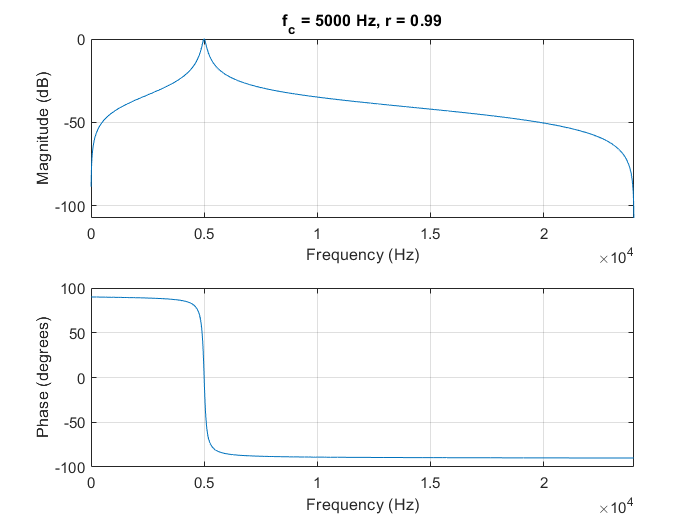
\includegraphics[scale=.53]{./images/plots/ResonatorTest.png}
    \caption{The measured frequency response for 2nd-order resonator test.}
    \label{fig:ResoTest}
\end{figure}

\subsection{DC Blocker}
The DC blocker is implemented with the following difference equation:
\begin{equation}
    y[n] = g (x[n] - x[n-1]) + Ry[n-1]
\end{equation}
where $g = \frac{1+R}{2}$. As there is a feedback term ($y[n-1]$), this is an IIR filter. Figure~\ref{fig:DCBlockerResponse} illustrates the DC blocker's frequency response for a value of $R = .995$.

\begin{figure}[h]
    \centering
    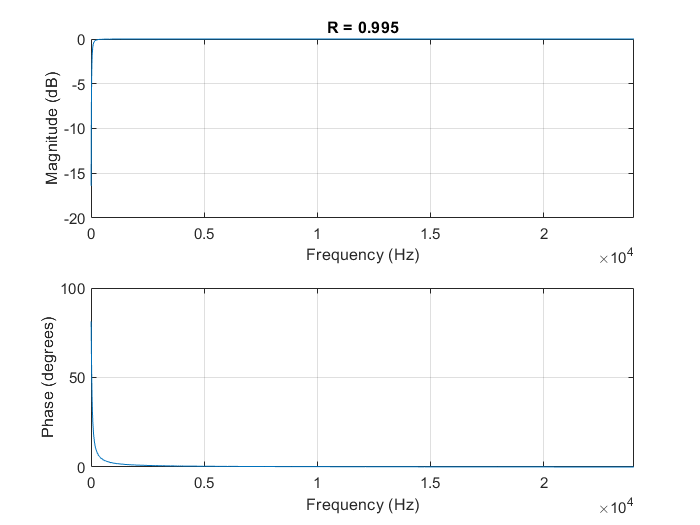
\includegraphics[scale=.53]{./images/plots/DCBlockerResponse.png}
    \caption{The measured frequency response for the DC Blocker test.}
    \label{fig:DCBlockerResponse}
\end{figure}

\subsection{Smoothing Filter}
\label{subsec:Ch4SmoothingFilter}
The smoothing filter is implemented via a 10-point moving average where every sample is weighted evenly. Its difference equation is:

\begin{equation}
    y[n] = \frac{1}{10} \sum_{m = 0}^{9}x[n-m]  
\end{equation}

This is verified by the output shown in Fig.~\ref{fig:SmoothingIR}. Extra elements are shown to indicate the filter outputs zeros after the 10th iteration (corresponding to $n = 9$). Given that it is easier to understand this filter from its impulse response, and this is paired to the frequency response via the Fourier Transform, verification for this was done in the time-domain.

\begin{figure}[!h]
    \centering
    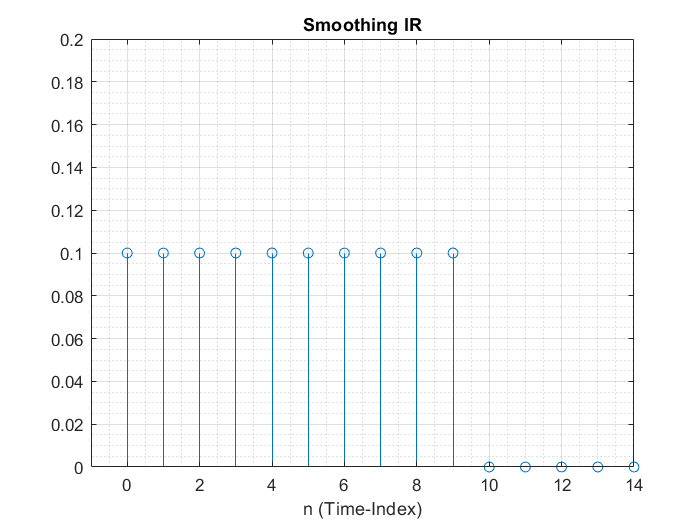
\includegraphics[scale=.53]{./images/plots/SmoothingIR.png}
    \caption{The impulse response of the implemented smoothing filter.}
    \label{fig:SmoothingIR}
\end{figure}

\subsection{Longitudinal Modes}
The precise method by which the longitudinal mode filters were derived and designed is not completely specified in either \citetwo{puputti_real-time_2010} or \citetwo{pakarinen_virtual_2008}. What is explained is that a linear-prediction filter of order 100 was used to estimate the spectrum of the different modes of each slide/wound string interaction. From this, a 4th-order IIR filter was derived based on the most prominent resonances. The pole/zero locations for these 4th-order filters are what is provided for an implementation. Only plots of the magnitude responses for the different filters as well as the linear-prediction estimates are provided. These plots are shown in Fig.~\ref{fig:LongModeOrig}. These 4th-order approximations were recreated for the implemented longitudinal mode filters as shown in Fig.~\ref{fig:LongModeRecr}. Verification was done through visual comparison of the plots as there is no data to easily facilitate computing an error function. 

In summary, all the filters work according to their expected behavior.

\begin{figure}[h]
        \centering
        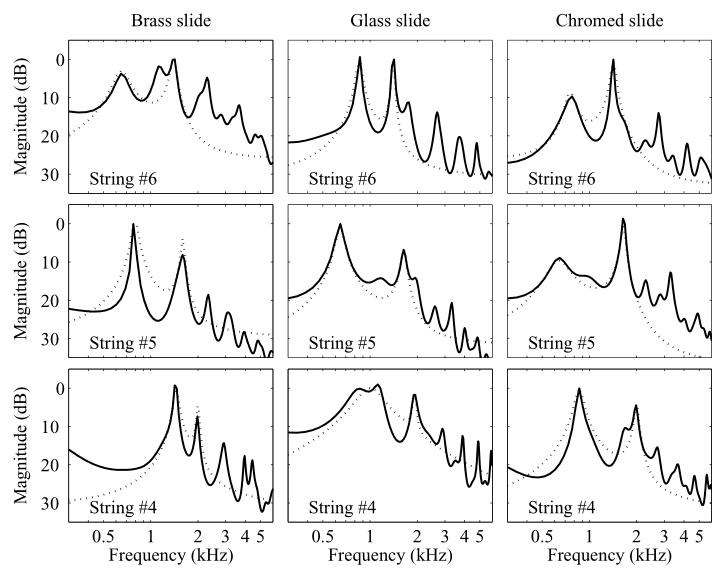
\includegraphics[scale=.65]{./images/plots/LongitudinalModeFiltersOriginal.png}
        \caption{Original figure from \citetwo{pakarinen_virtual_2008} for comparison purposes. Solid lines represent spectral estimates using linear-prediction filter of order 100. Dotted lines indicate modal filter magnitude responses.}
        \label{fig:LongModeOrig}
\end{figure}

\begin{figure}[h]
        \centering
        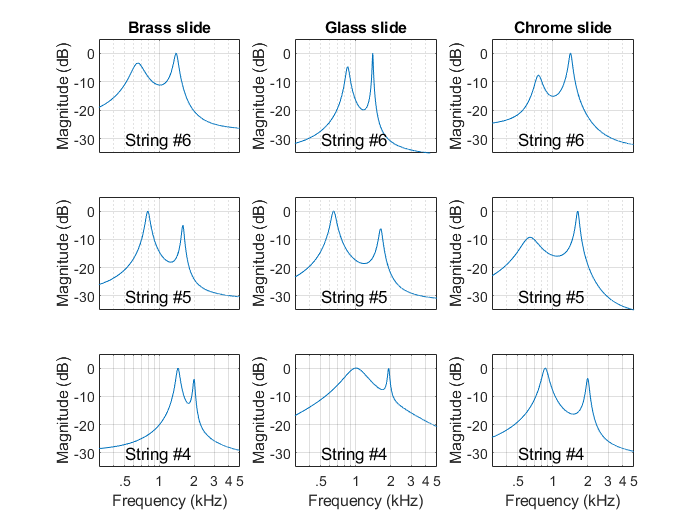
\includegraphics[scale=.65]{./images/plots/LongitudinalModeFiltersRecreation.png}
        \caption{The implemented longitudinal mode filters' magnitude responses. These correspond to the dotted lines of Fig.~\ref{fig:LongModeOrig}.}
        \label{fig:LongModeRecr}
\end{figure}

\section{Control Signal Processor}
The Control Signal Processor (see Sec.~\ref{subsec:Ch3ControlSignalProcessor}) consists of three components:
\begin{enumerate}
    \item \textbf{Slide Speed Extractor} - This block performs numerical differentiation on the relative length signal followed by an absolute-value to generate the slide speed control signal.
    \item \textbf{Interpolator} - This block performs linear interpolation to upsample control rate signals to the audio rate.
    \item \textbf{Smoothing Filter} - This block smooths the interpolated signals to mitigate any discontinuities introduced during processing.
\end{enumerate}
The Smoothing Filter was verified earlier in Sec.~\ref{subsec:Ch4SmoothingFilter}. What remains to be shown is that the Interpolator and Slide Speed Extractor operate correctly as well as the Control Signal Processor as a whole, given that it is created by the interconnection of these components.

\subsection{Components of Control Signal Processor}
\subsubsection{Interpolator}
The interpolator block operates via linear interpolation.  It was tested by specifying a control signal $L[m]$ and running it through the interpolator. Figure~\ref{fig:InterpTest} illustrates this. The original $L[m]$ is plotted with black *. The interpolated $L[n]$ output is plotted as red circles with linear line segments to help ensure linear trajectories were maintained. Red and black are used to help disambiguate the input and output. For this figure, the audio rate was specified as 48,000 Hz while the control rate was specified as 12,000 Hz. This would give a ratio of $R = \frac{48000}{12000} = 4$, meaning 3 interpolated audio samples would need to be calculated for every 1 control sample. $R$ can only take on integer values. It is also necessary to specify an initial value for the interpolation to start from. In this figure, $0.5$ was used for the initial value. As is shown, the linear interpolation is performed correctly.

\begin{figure}[h]
    \centering
    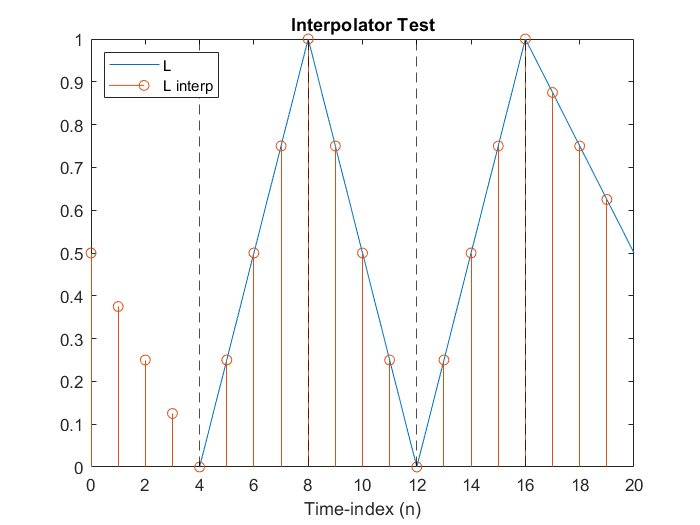
\includegraphics[scale=.65]{./images/plots/InterpolatorTest.png}
    \caption{The output from the Interpolator test. The black axes and * represent the original control rate signal. The red axes and circles represent the interpolated output. Line segments have been added to help illustrate the linearity. The initial value used to start the interpolation is 0.5 and R = 4. The different colors are to help disambiguate input from output.}
    \label{fig:InterpTest}
\end{figure}

\subsubsection{Slide Speed Extractor}
\label{sec:SSE_test}
The Slide Speed Extractor was tested by taking a theoretical curve which represents a parabolic $slideSpeed[n]$ trajectory. From this, the corresponding relative length signal for a specified string length was generated using the equation:
\begin{equation}
    L[n] = L[n-1] - \frac{slideSpeed[n]}{F_s \times StringLength}
\end{equation}
This curve was then fed into the Slide Speed Extractor object to generate the corresponding $slideSpeed[n]$. The error between the theoretical and measured values was calculated. The output of this is shown in Fig.~\ref{fig:SlideSpeedTest}. Given that the error signal is a constant 0, this illustrates correct operation of the slide signal extractor.

\begin{figure}[h]
    \centering
    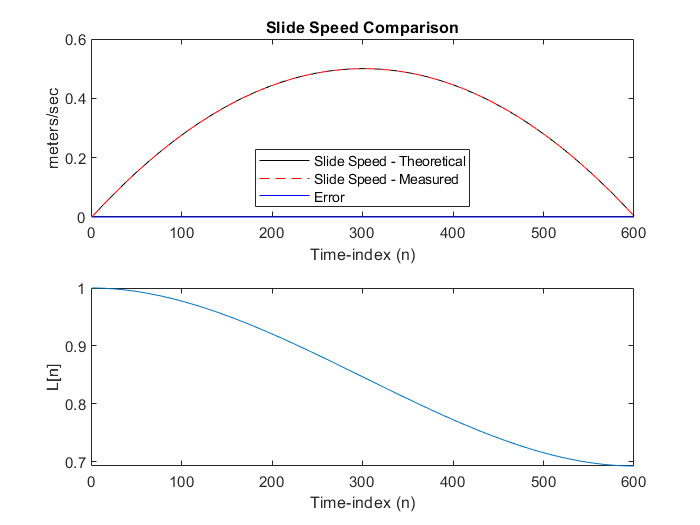
\includegraphics[scale=.65]{./images/plots/SlideSpeedExtractorTest.png}
    \caption{The top plot illustrates the correctness of the slide speed extraction algorithm while the lower plot displays the $L[n]$ signal which was used as a stimuli.}
    \label{fig:SlideSpeedTest}
\end{figure}

\subsection{Control Signal Processor as a Whole}
With the constituent components verified as working, the test here confirms that everything is linked together correctly inside the Control Signal Processor. Figure~\ref{fig:CSPTest} illustrates the output of the Control Signal Processor to a specified $L[m]$ control signal. This was chosen to be linear to make the interpolation and smoothing easier to verify. The $slideSpeed[n]$ signal can be seen as indicating the slide starts from rest and then gradually ramps up to constant speed. This is consistent with what would be expected as we have specified that the starting $L[m]$ value in the Control Signal Processor corresponds to when $m = 0$.

\begin{figure}[h]
    \centering
    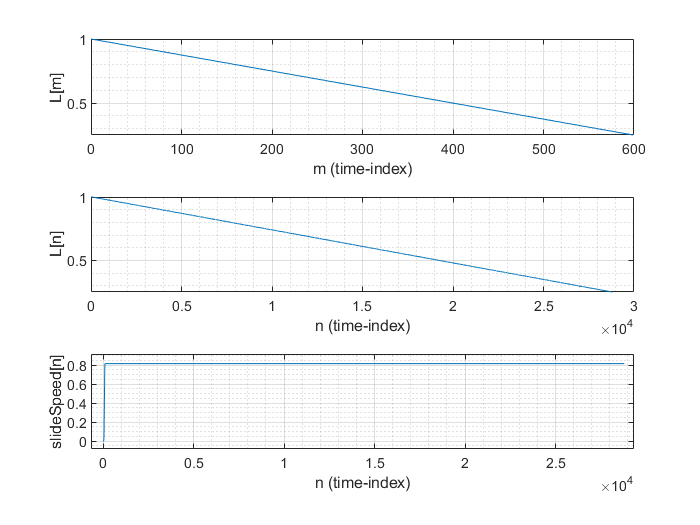
\includegraphics[scale=.65]{./images/plots/CSPTest.png}
    \caption{The $L[m]$ input signal and corresponding output signals for CSP test.}
    \label{fig:CSPTest}
\end{figure}

\section{Noise Generation Objects}
\subsection{Impulse Train}
The Impulse Train object responds to the $f_c[n]$ signal which controls its firing rate. Accordingly, various artificial $f_c[n]$ signals were generated to ensure the different run-time use cases would execute correctly during synthesis. These test are:
\begin{enumerate}
    \item $f_c[n]$ is a constant during operation and impulses are generated at regular intervals.
    \item $f_c[n]$ decreases during operation and the number of samples between impulses increases.
    \item $f_c[n]$ increases during operation and the number of samples between impulses decreases.
    \item $f_c[n]$ is set to zero during operation and no more impulses are produced .
    \item $f_c[n]$ changes from 0 to a positive value and impulses begin being produced.
\end{enumerate}
The full details can be found in the link in Appendix~\ref{apen:CodeAndSound}. The different test cases are illustrated in the same order in Fig.~\ref{fig:ImpulseTrainTest}. As can be seen in the figure, the Impulse Train object operates as expected. 

\begin{figure}[h]
    \centering
    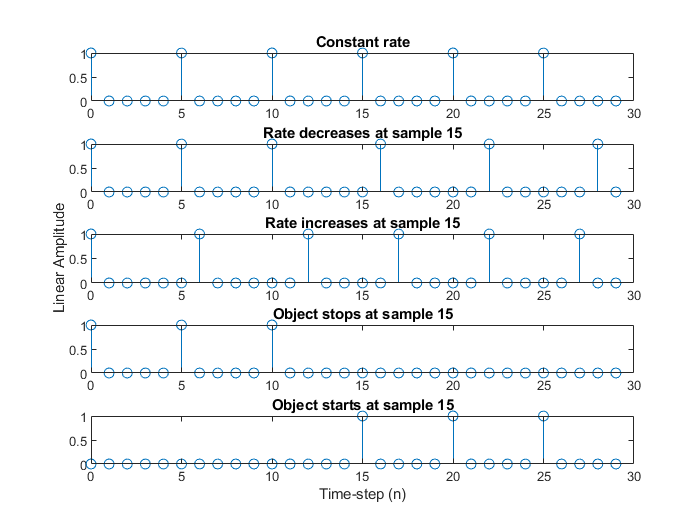
\includegraphics[scale=.65]{./images/plots/ImpulseTrainTest.png}
    \caption{The Impulse Train test output.}
    \label{fig:ImpulseTrainTest}
\end{figure}

\subsection{Exponential Decay}
The Exponential Decay object is composed of an Impulse Train which excites a one-pole filter whose feedback coefficient is tuned to match the specified $T_{60}$ parameter. As the Impulse Train was tested separately, it was necessary to ensure that the $T_{60}$ parameter was implemented correctly. Figure~\ref{fig:ExpDecayTest1} illustrates correct functioning of the Exponential Decay object for three different $T_{60}$ values. The plots illustrate the envelopes generated by the Exponential Decay. The $T_{60}$ were initially specified as $\frac{1}{4}$ seconds, $\frac{1}{8}$ seconds and $\frac{1}{16}$ seconds. The dB scale is used for the y-axis to make it easier to identify the point where the envelope has decayed by 60 dB. The $T_{60}$ values have been converted into samples by multiplication with $F_s = 48,000$ kHz, to allow for easier verification.

\begin{figure}[ht]
    \centering
    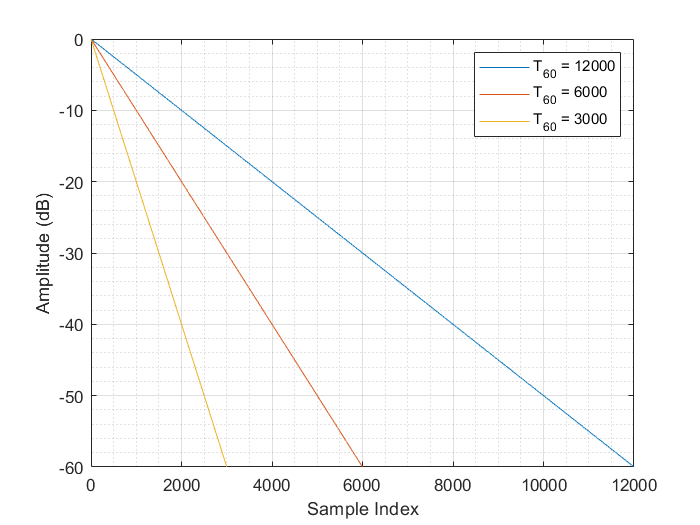
\includegraphics[scale=.65]{./images/plots/ExpDecayTest1.png}
    \caption{The test results for three different $T_{60}$ decay parameters specified in samples.}
    \label{fig:ExpDecayTest1}
\end{figure}

\clearpage
 
\subsection{Noise Pulse Train}
The Noise Pulse Train object was tested with two different scenarios: a constant firing rate producing 12 distinct pulses with no overlap and a swept firing rate corresponding to the same parabolic trajectory used to verify the Slide Speed Extractor in Sec.~\ref{sec:SSE_test}. The results are illustrated in Figs.~\ref{fig:NPTT1}-\ref{fig:NPTT2Spec}. Note the overlap of the individual pulses in the second test due to the firing rate being faster than the decay rate. This overlap causes the signal to become more noise-like. The spectrum also illustrates how the signal has a harmonic component in the lower end. The output of each test can be heard in the files \emph{NoisePulseTrain-test1.wav} and \emph{NoisePulseTrain-test2.wav}. Through these examples, as well as their spectrograms, the Noise Pulse Train object has been verified as working correctly both subjectively and objectively. The ``noisiness" of a signal at higher values of $f_c$ can be controlled by the $T_{60}$ parameter as will be discussed in Sec.~\ref{subsec:Ch6DecayRate}.

\begin{figure}[h!]
    \centering
    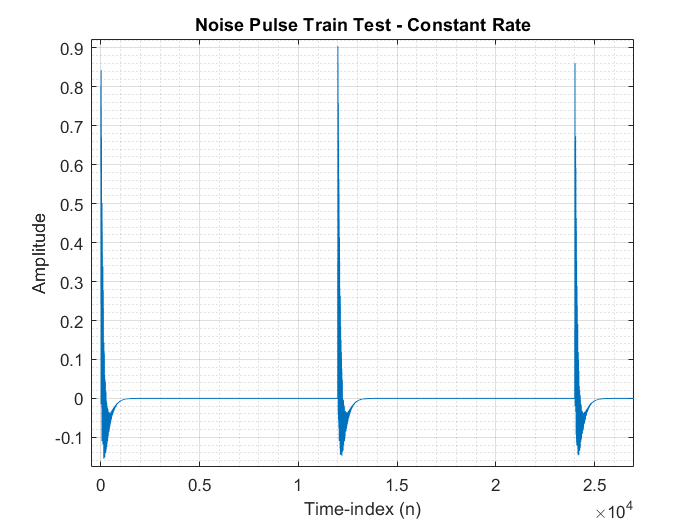
\includegraphics[scale=.65]{./images/plots/NPTTest1.png}
    \caption{The Noise Pulse Train output for a constant rate. Note the negative values introduced by the DC Blocker. These have no perceptual impact, but is a deviation from the original design described in \citetwo{pakarinen_virtual_2008}.}
    \label{fig:NPTT1}
\end{figure}

\clearpage

\begin{figure}[h!]
    \centering
    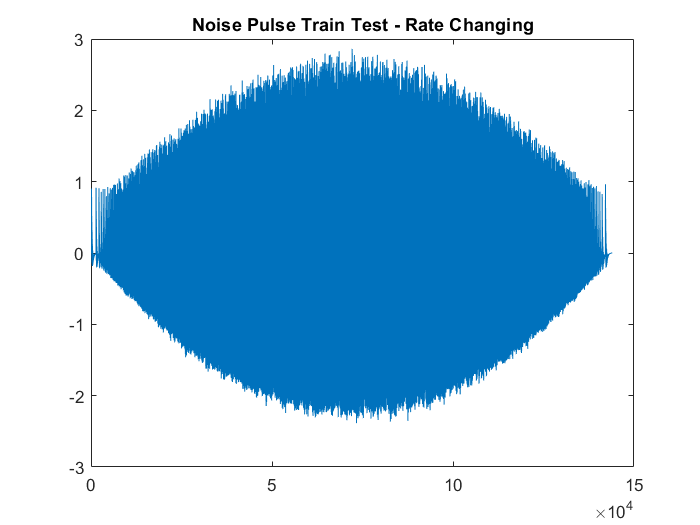
\includegraphics[scale=.60]{./images/plots/NPTTest2.png}
    \caption{The Noise Pulse Train output in response to an $f_c[n]$ sweep. Note the overlapping build-up of the individual impulses. Individual pulses can be seen at the ends.}
    \label{fig:NPTT2}
\end{figure}

\begin{figure}[h!]
    \centering
    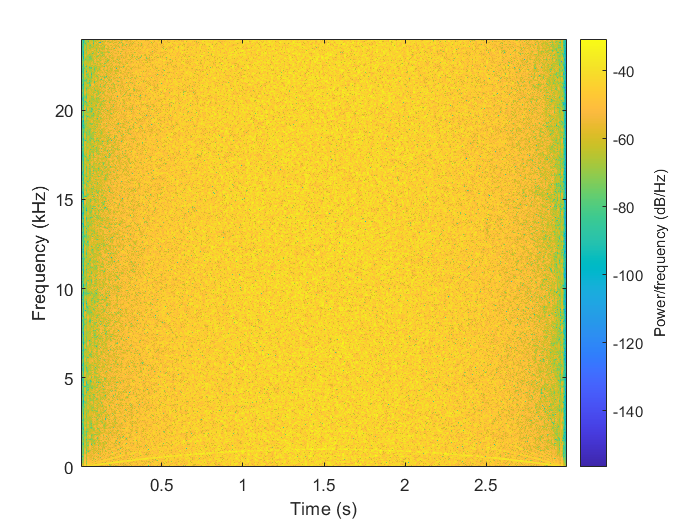
\includegraphics[scale=.60]{./images/plots/NPTTest2Spectrum.png}
    \caption{This spectrum corresponds to Fig.~\ref{fig:NPTT2}. Note the emergence of harmonics at the lower end as compared to the results shown in Fig.~\ref{fig:NBGT2}.}
    \label{fig:NPTT2Spec}
\end{figure}

\clearpage

\subsection{Noise Burst Generator}
\label{sec:NBGVerify}
The Noise Burst generator was tested with the same two input signals as the Noise Pulse Train. The outputs are shown in Figs.~\ref{fig:NBGT1}-\ref{fig:NBGT2Spec}. The sounds can be heard in the files \emph{NoiseBurstGen-test1.wav} and \emph{NoiseBurstGen-test2.wav}. The noisiness in the second example was by design as explained in Sec.~\ref{subpara:Ch3NBG}. Each of the different noise sources were originally designed to work with only one of the Harmonic Accentuation techniques described in Sec.~\ref{subsec:WoundString}. The Noise Burst Generator operates best with the Harmonic Resonator Bank as will be elaborated upon in Sec.~\ref{subsec:NS_and_HA_Combos}.

\begin{figure}[hb]
    \centering
    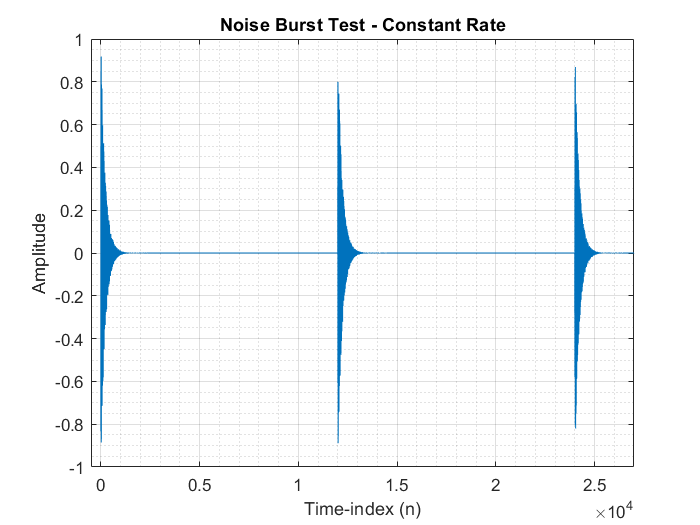
\includegraphics[scale=.65]{./images/plots/NBGTest1.png}
    \caption{The Noise Burst Generator output for a constant rate. Note the approximate symmetry about the x-axis. The symmetry eliminates the need for a DC blocker.}
    \label{fig:NBGT1}
\end{figure}

\begin{figure}[ht]
    \centering
    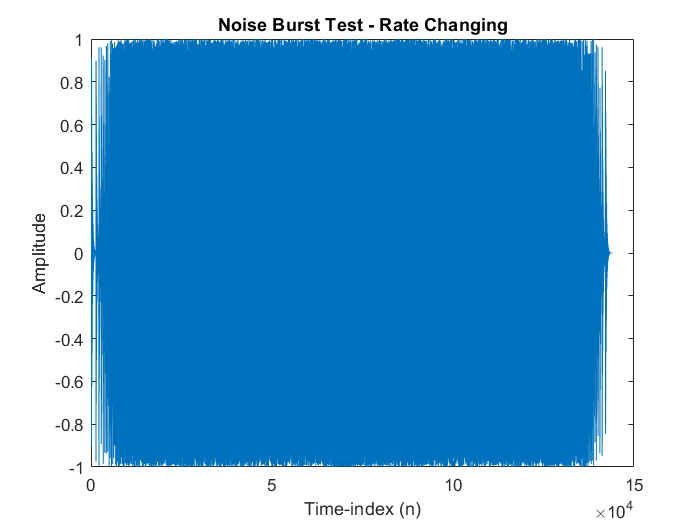
\includegraphics[scale=.65]{./images/plots/NBGTest2.png}
    \caption{The Noise Burst Generator output in response to an $f_c[n]$ sweep. Note the effects of the hard-clipping and how the signal transitions into noise as was intended.}
    \label{fig:NBGT2}
\end{figure}

\begin{figure}[hb]
    \centering
    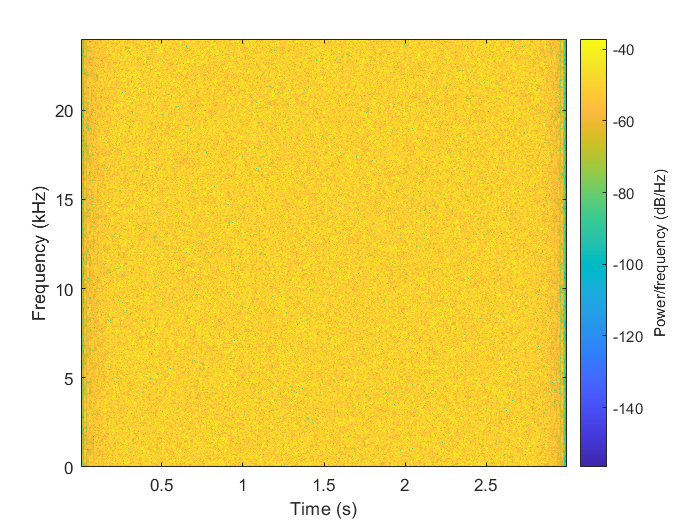
\includegraphics[scale=.65]{./images/plots/NBGTest2Spectrum.png}
    \caption{The spectrum corresponding to Fig.~\ref{fig:NBGT2}. Note the lack of harmonics as compared to Fig.\ref{fig:NPTT2}.}
    \label{fig:NBGT2Spec}
\end{figure}

\clearpage

\section{Harmonic Accentuators}
\subsection{Harmonic Resonator Bank}
Given that the resonators were verified in Sec.~\ref{subsec:resoTest}, the Harmonic Resonator Bank was verified by running white noise through the system while performing a sweep on the $f_c$ control parameter. The sweep follows the same parabolic trajectory from Sec.~\ref{sec:SSE_test}. The functionality of this block predicts that we would observe six harmonically linked bands in the output spectrum. This is shown in Fig.~\ref{fig:HRBTest} where the different harmonics' trajectories are overlaid in red. The output can be heard in \emph{HRB-test.wav}. Both the recording and spectrogram provide objective and subjective evidence that the Harmonic Resonator Bank works as is expected and is free from unwanted artifacts.

\begin{figure}[h]
    \centering
    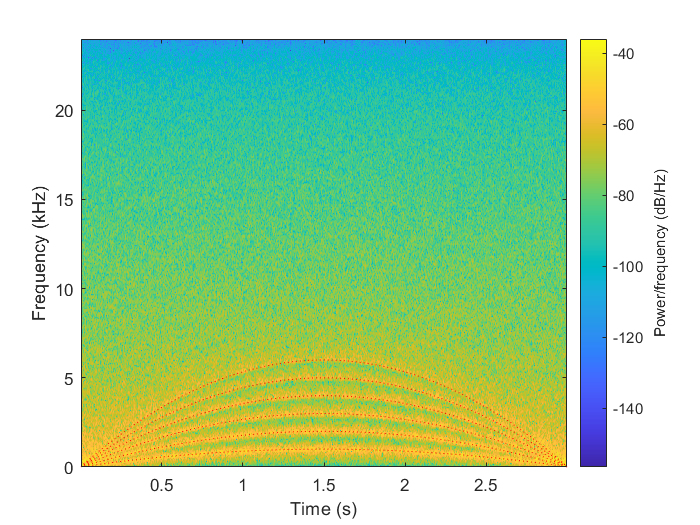
\includegraphics[scale=.65]{./images/plots/HRBTest.png}
    \caption{The output from Harmonic Resonator Bank test. The dotted red lines indicate the theoretical harmonic trajectories.}
    \label{fig:HRBTest}
\end{figure}

\subsection{Reso + Tanh}
The Reso + Tanh block (Sec.~\ref{subpar:Ch3Reso+Tanh}) was tested using the same $f_c$ sweep. The stimuli was changed to use the Noise Pulse Train object instead as the $\tanh()$ function relies on a periodic signal being input in order to achieve the desired effect of accentuating/creating harmonics. Figure~\ref{fig:ResoTanhTest} illustrates the output spectrum from the test. Note the much finer concentration of energy in the harmonic bands, the emphasis of the fundamental due to the different noise source and more than 6 harmonics being generated. This helps provide a finer sense of perceptual fusion for the generated sound. The output of this can be heard in \emph{ResoTanh-test.wav}.

\begin{figure}[h]
    \centering
    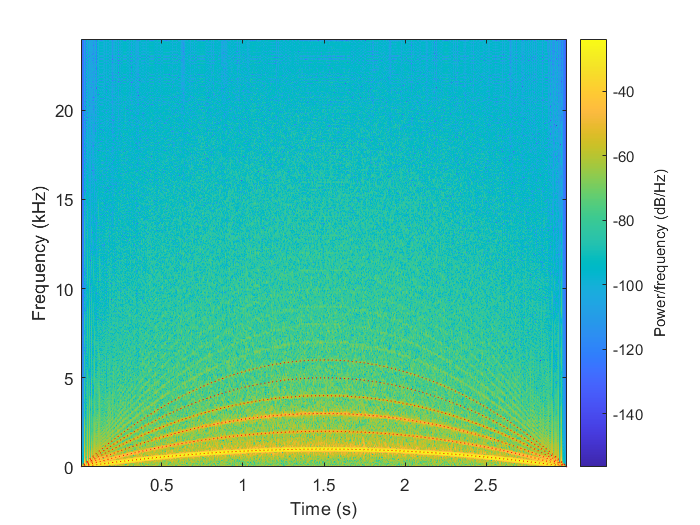
\includegraphics[scale=.65]{./images/plots/ResoTanhTest.png}
    \caption{The output from Reso + Tanh test. The dotted red lines indicate the theoretical harmonic trajectories.}
    \label{fig:ResoTanhTest}
\end{figure}

\section{Contact Sound Generator (CSG)}
Both the wound and unwound CSGs were verified using the following three test cases based on the qualities of the slide motion:

\begin{enumerate}
    \item No slide motion
    \item Slide motion with a constant slide velocity
    \item Slide motion with a time-varying slide velocity
\end{enumerate}

These were selected as they covered the basic use cases which would arise during synthesis. The constant slide velocity test uses a slide velocity which generates an $f_c[n]$ of 250 Hz. The time-varying slide velocity is configured to generate a parabolic sweep of $f_c[n]$ from 0 Hz to 1kHz and back to 0 Hz (as with the previous similar tests). This mimics the speed experienced by a slide which starts at rest and moves between two positions on the fingerboard. Test scenario 1 (no slide motion) is mentioned for completeness purposes. Results and figures from that test will not be discussed due to its simplicity.

\subsection{Wound Variant}
The audio producing tests were further sub-divided into three other tests by controlling the balance between the two sound components. This was done to ensure proper functioning of each branch as well as help determine each branch's audible contribution in the combined sound. As part of the sound design process, the four different combinations of noise sources and harmonic accentuation techniques were tested (as will be elaborated upon in the Sound Design chapter). The following figures were generated using the Noise Pulse Train and Harmonic Resonator Branch configuration in order to reduce the total number of figures.

\begin{enumerate}
    \item Longitudinal branch isolated
    \item Harmonic branch isolated
    \item Both branches combined
\end{enumerate}

In the spectrograms showing the results, the dashed black lines represent the specified longitudinal mode frequencies and the dotted red lines indicate the theoretical harmonic trajectories.

\subsubsection{Static $f_c[n]$}
The results for the constant slide velocity scenario are shown in Figures~\ref{fig:CSGWoundStaticLong}-\ref{fig:CSGWoundStaticBoth}. Figure~\ref{fig:CSGWoundStaticLong} illustrates how the original source stimuli produced by the Noise Pulse Generator does not contain strong frequency components at the 1st longitudinal mode frequency. Also illustrated is that the harmonic branch extracts and emphasizes the fundamental while retaining many of the upper harmonics in decreasing strength. The corresponding audio can be heard in \emph{CSG-Wound-Static-Long.wav}, \emph{CSG-Wound-Static-Harm.wav} and \emph{CSG-Wound-Static-Both.wav}.

\begin{figure}[h!]
    \centering
    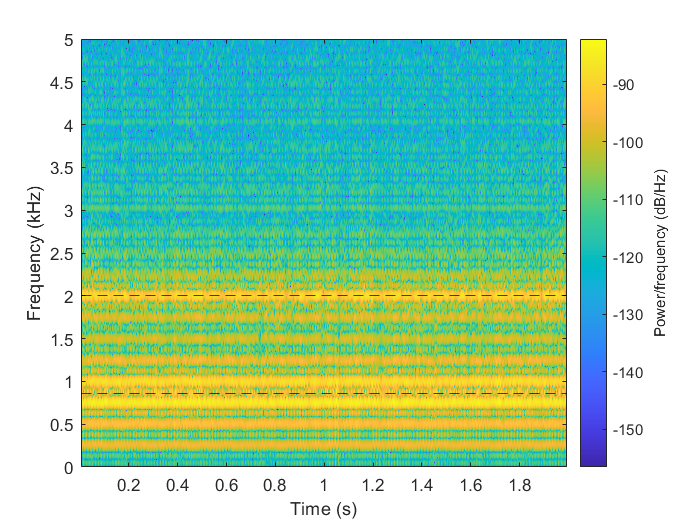
\includegraphics[scale=.57]{./images/plots/CSG_Wound_Static_Long.png}
    \caption{The output from the Wound CSG test using a static slide velocity for the longitudinal branch ($v_1[n]$ in Fig.~\ref{fig:CSG_wound}). The dashed black lines indicate longitudinal mode frequencies. As the stimuli does not contain frequencies near the first mode, there is less energy there.}
    \label{fig:CSGWoundStaticLong}
\end{figure}

\begin{figure}[h!]
    \centering
    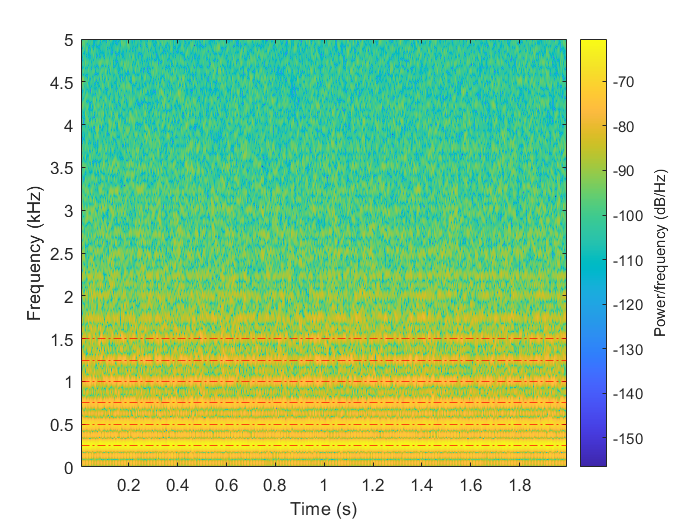
\includegraphics[scale=.60]{./images/plots/CSG_Wound_Static_Harm.png}
    \caption{The output from the Wound CSG test using a static slide velocity for the harmonic branch ($v_2[n]$ in Fig.~\ref{fig:CSG_wound}). The dotted-dashed red lines indicate the frequencies for the first six harmonics.}
    \label{fig:CSGWoundStaticHarm}
\end{figure}

\begin{figure}[h!]
    \centering
    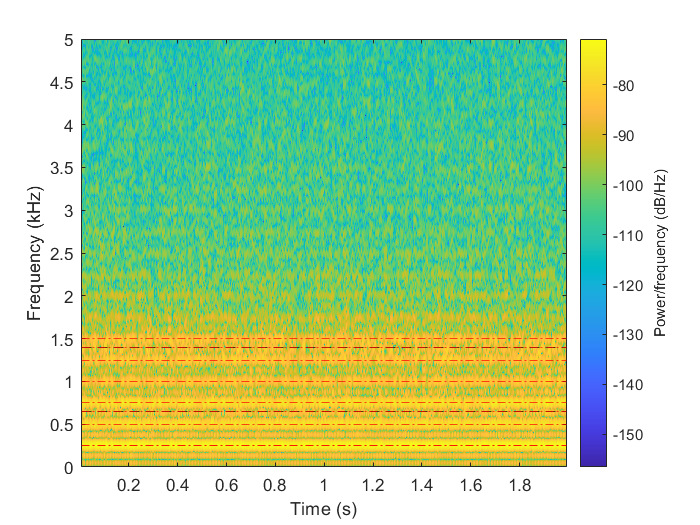
\includegraphics[scale=.60]{./images/plots/CSG_Wound_Static_Both.png}
    \caption{The output from the Wound CSG test using a static slide velocity for both combined branches. Notice how this is a combination of Fig.~\ref{fig:CSGWoundStaticLong} and Fig.~\ref{fig:CSGWoundStaticHarm}.}
    \label{fig:CSGWoundStaticBoth}
\end{figure}

\subsubsection{Time-Varying $f_c[n]$}
The results for the time-varying slide velocity scenario are shown in Fig.~\ref{fig:CSGWoundTVLong}-\ref{fig:CSGWoundTVBoth}. Dashed red lines indicate the theoretical harmonic trajectories. Dashed blacked lines correspond to the static longitudinal modes. As is clearly shown in Fig.~\ref{fig:CSGWoundTVLong}, the longitudinal modes are only stimulated when the frequencies the filters are tuned to are present in the incoming signal. It also illustrates how some of the harmonic components leak through, which will be reinforced when added to the output from the harmonic branch. Only $\frac{1}{3}$ of the spectrum is plotted to emphasize these points. The corresponding audio can be heard in \emph{CSG-Wound-TV-Long.wav}, \emph{CSG-Wound-TV-Harm.wav} and \emph{CSG-Wound-TV-Both.wav}.

\begin{figure}[hb]
    \centering
    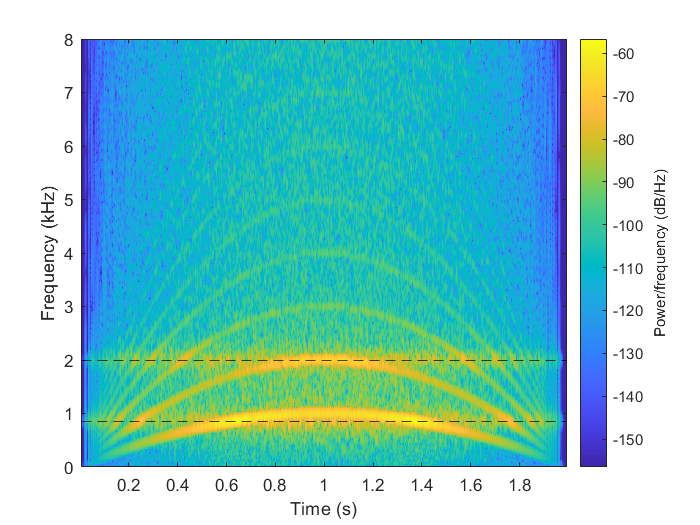
\includegraphics[scale=.65]{./images/plots/CSG_Wound_TV_Long.png}
    \caption{The output from the Wound CSG test using a time-varying slide velocity for the longitudinal branch. The dashed black lines indicate longitudinal mode frequencies. When the fundamental of the sweep matches a modal frequency it is reinforced more.}
    \label{fig:CSGWoundTVLong}
\end{figure}

\begin{figure}[t]
    \centering
    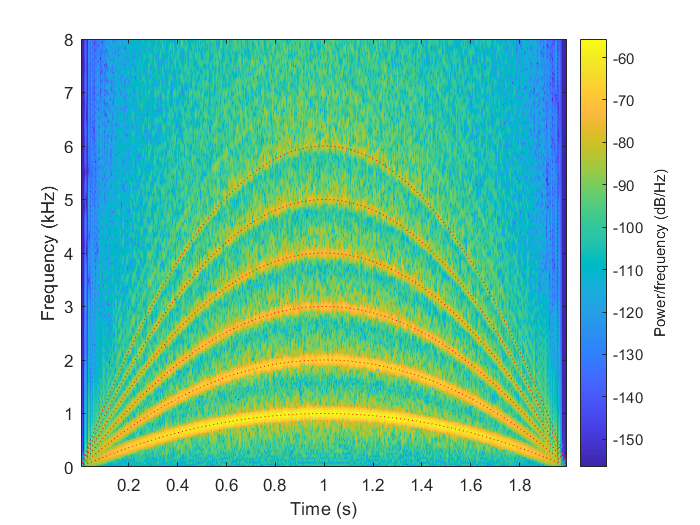
\includegraphics[scale=.60]{./images/plots/CSG_Wound_TV_Harm.png}
    \caption{The output from the Wound CSG test using a time-varying slide velocity for the harmonic branch. The dotted red lines indicate the frequencies for the first six harmonics.}
    \label{fig:CSGWoundTVHarm}
\end{figure}

\begin{figure}[b]
    \centering
    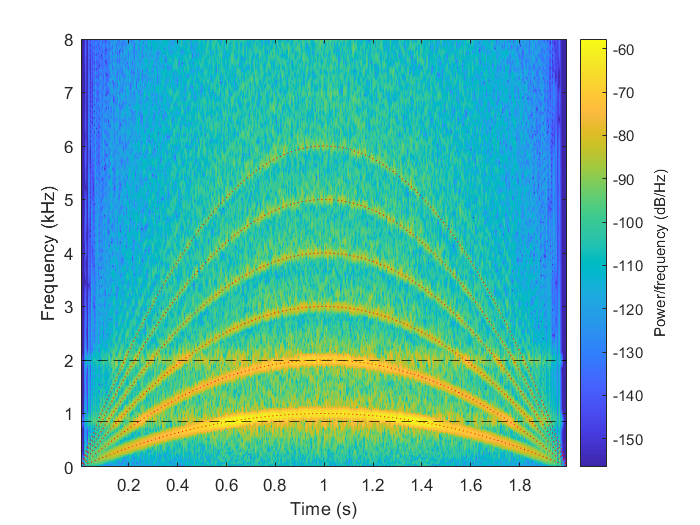
\includegraphics[scale=.60]{./images/plots/CSG_Wound_TV_Both.png}
    \caption{The output from the Wound CSG test using a static slide velocity for both combined branches. Notice how this is a combination of Fig.~\ref{fig:CSGWoundTVLong} and Fig.~\ref{fig:CSGWoundTVHarm}.}
    \label{fig:CSGWoundTVBoth}
\end{figure}

\clearpage

\subsection{Unwound Variant}
Figure~\ref{fig:CSGUnwoundTVSpec} illustrates the output of the unwound Contact Sound Generator for the same time-varying slide speed signal. It is substantially less interesting but still necessary for the purposes of verification. As can be seen, the low-pass filter applied creates a roll-off at the top of the spectrum while the ramp-in and ramp-down create the variations in spectral energy near the beginning and end of the sound. This can be heard in the file \emph{CSG-Unwound-TV.wav}. The rest of the scenarios were also run on this module but are not shown here.

\begin{figure}[h]
    \centering
    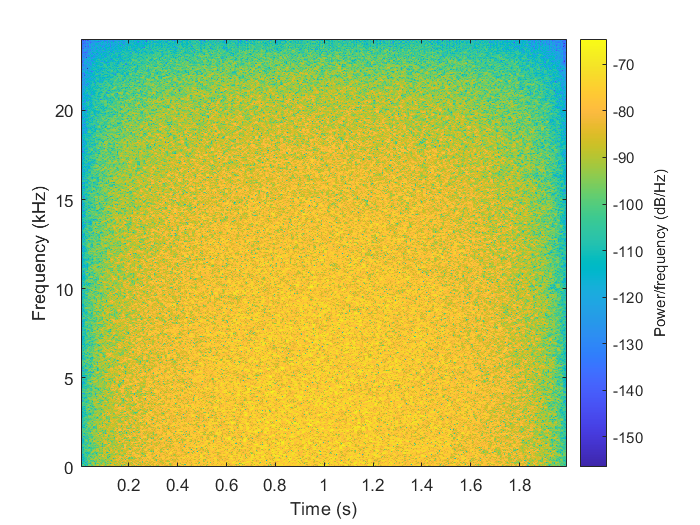
\includegraphics[scale=.65]{./images/plots/CSG_Unwound_TV.png}
    \caption{The output from unwound branch for time-varying slide velocity.}
    \label{fig:CSGUnwoundTVSpec}
\end{figure}

\section{String DWG and its Components}

\subsection{Interpolated Delay Line}
The core-class which this object was built around is a circular buffer. The circular buffer class was tested thoroughly itself (see source code). Illustrated here is the verification of the Lagrange interpolation as this is crucial to ensuring the correct functioning of the synthesis algorithm. In this test, $D$ represents the nominal delay implemented by the Lagrange interpolator. It can also be expressed as $D = \lfloor D \rfloor + d$, where $d$ is the fractional component. The order of the Lagrange interpolator is set to 5. At this order, $D$ could take values on the interval $[0,5)$ samples. However, Lagrange interpolation works best near the mid-point so $D$ is constrained to $[2, 3)$. $M$ represents delay in samples as implemented by the integer delay line, which precedes the Lagrange interpolator in the overall interpolated delay line structure. See \ref{fig:LagrangeStructure} for reference. Given that the order of the Lagrange interpolator creates a lower bound on the length of the interpolated delay line, limits are set based on a specified highest-fret (which results in a minimum $L[n]$) to ensure this lower bound is avoided.

The first test that was performed was a test to ensure that it could indeed operate as an integer delay. Various Interpolated Delay Line objects were constructed, ensuring that no fractional delay would be required. The output of this test is shown in Fig.~\ref{fig:LagrangeTest1} where $x$ is the input signal and $y$ is the output. As this figure clearly shows, the interpolated delay line clearly implements this functionality.

\begin{figure}[h]
    \centering
    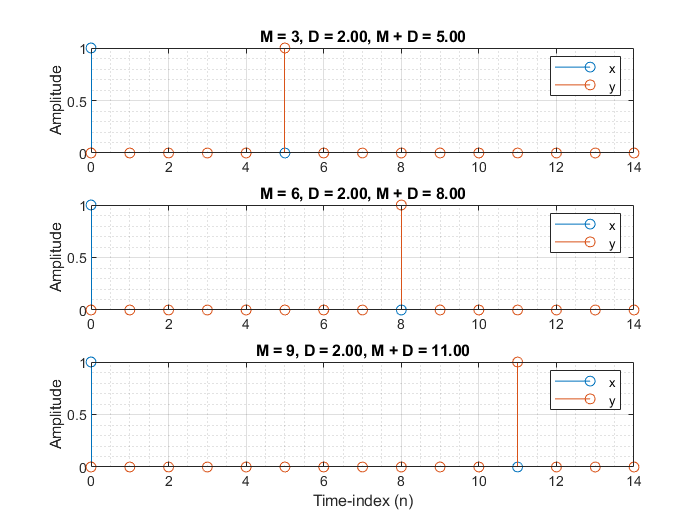
\includegraphics[scale=.65]{./images/plots/LagrangeTest1.png}
    \caption{The test results of integer values for the interpolated delay line object. $x[n]$ is the input impulse stimuli and $y[n]$ is the resulting delayed output. The delay values are indicated above each plot.}
    \label{fig:LagrangeTest1}
\end{figure}

The second test which was performed ensures that the delay line value can be updated during the run-time. This differs from the previous test where a new object was constructed each time. Figure~\ref{fig:LagrangeTest2} illustrates this test. The delay line starts out with an initial delay of 10 samples. After 15 samples have passed this is incremented by 1. After another 15 samples have passed this is decremented by two. Impulses are fed into the delay line every 15 samples to show the changes.

\begin{figure}[h]
    \centering
    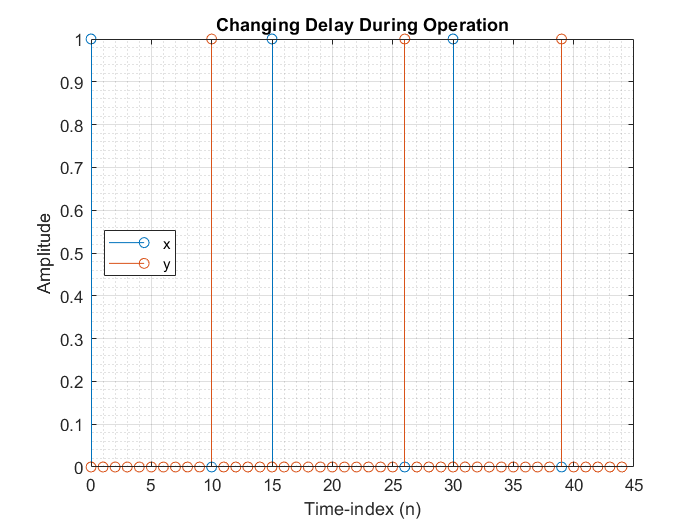
\includegraphics[scale=.65]{./images/plots/LagrangeTest2.png}
    \caption{$x[n]$ is an impulse train with a period of 15 samples and $y[n]$ represents the delay line output. The delay value starts at 10, increases to 11 at $n = 15$ and decreases to 9 at $n = 30$. This illustrates that the interpolated delay line can change delay values during operation.}
    \label{fig:LagrangeTest2}
\end{figure}

The third test which was performed is similar to the second, however now the fractional component was changed to ensure the coefficients of the Lagrange FIR are calculated correctly. Table~\ref{tab:LagrangeTest3} illustrates the parameter changes which occur every 15 samples. Under these conditions, the length of the interpolation filter is 6 samples, while $M$ is 8 samples. The output of this test is shown in Fig.~\ref{fig:LagrangeTest3}. As is clearly shown, the impulse response of the Lagrange interpolator, corresponding to the different fractional delays, appears in the six samples after the eight zeros (which correspond to the integer delay component of the structure).

\begin{figure}[h!]
    \centering
    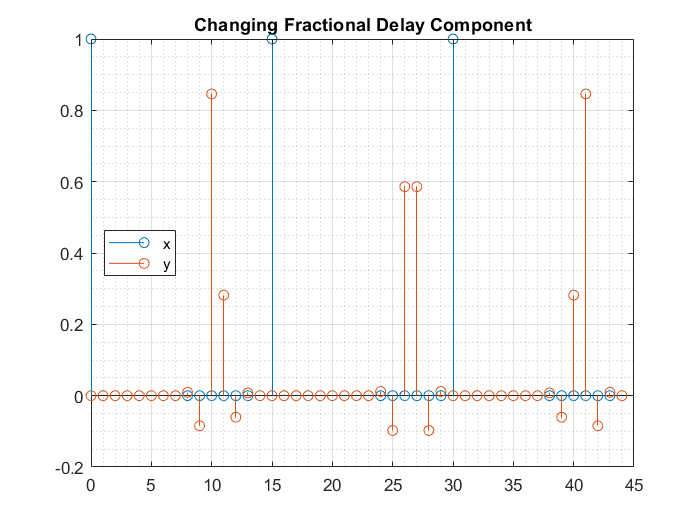
\includegraphics[scale=.65]{./images/plots/LagrangeTest3.png}
    \caption{$x[n]$ is an impulse train with a period of 15 samples used as input. $y[n]$ is the corresponding output. The parameter changes are specified in Table~\ref{tab:LagrangeTest3}. The output illustrates the appropriate number of integer delay values followed by the impulse response of a filter approximating the Lagrange interpolation.}
    \label{fig:LagrangeTest3}
\end{figure}

\begin{table}[h!]
    \centering
     \begin{tabular}{||c| |c |c |c|} 
         \hline
         \textbf{n} & \textbf{M} & \textbf{d} & \textbf{D} \\ [0.5ex] 
         \hline
         0 & 8 & .25 & 10.25 \\ 
         \hline
         15 & 9 & .50 & 11.5 \\
         \hline
         30 & 8 & .75 & 10.75 \\
         \hline
    \end{tabular}
    \caption{The parameter changes for the test shown in Fig.\ref{fig:LagrangeTest3}.}
    \label{tab:LagrangeTest3}
\end{table}

\subsection{Energy Scaler}
The energy scaling coefficient (Sec.~\ref{subsec:Ch3EnergyScaler}) is governed by the following equation:
\begin{equation}
\label{eq:g_c_n}
    g_c[n] = \sqrt{1-\Delta x[n]}
\end{equation}
where $\Delta x[n]$ is the change in the length of the digital waveguide, in samples, at time-step $n$. Testing of this block was done by specifying two different curves representing the digital waveguide length in samples over time. As $x[n]$ could take an infinite variety of different sorts of functions, it was decided to limit the curves to be linear and quadratic. The theoretical output of what the energy scaler should produce was derived and then the output error was calculated by subtracting the measured results from the derived results.

Assuming we start with a continuous signal, a quadratic DWG length signal can be expressed as:
\begin{equation}
    DWGLength(t) = at^2 + c 
\end{equation}
Given $c = DWGLength(0)$,  the starting point of the sweep, then $a$ can be expressed as:
\begin{equation}
    a = \frac{sweepEnd - sweepStart}{sweepDuration^2}
\end{equation}
The continuous signal can then be sampled to produce the following discrete-time expressions:
\begin{align}
    DWGLength[n] = DWGLength(nT_s) = a(nT_s)^2 + c\\
    DWGLength[n-1] = a(n^2 - 2n + 1)T_s^2 + c
\end{align}
Given that $\Delta x = DWGLength[n] - DWGLength[n-1]$, we can express $g_c[n]$ as:
\begin{equation}
    g_c[n] = \sqrt{|1-a(2n-1)T_s^2|}
\end{equation}
and use the expressions for $a$ and $c$ to develop a parameterized theoretical curve for the ideal output to a quadratic input. A similar procedure can be followed for the simpler linear case.

Figures~\ref{fig:EnergyScalerLinInc} and~\ref{fig:EnergyScalerQuadInc} show the results for the linear and quadratic DWG Length functions respectively. The output to a linearly increasing function is a constant gain factor less than one. Based on Eq.~\ref{eq:g_c_n}, this is expected. $\Delta x$ for a linearly increasing DWG Length is a positive constant, making $g_c[n]$ on the interval $[0, 1)$. 

Figures~\ref{fig:EnergyScalerLinDec} and~\ref{fig:EnergyScalerQuadDec} illustrate the output to the same functions which are now decreasing. As is illustrated, the absolute error remains zero and the gain operates in the same pattern but applying amplification.

\begin{figure}[h!]
    \centering
    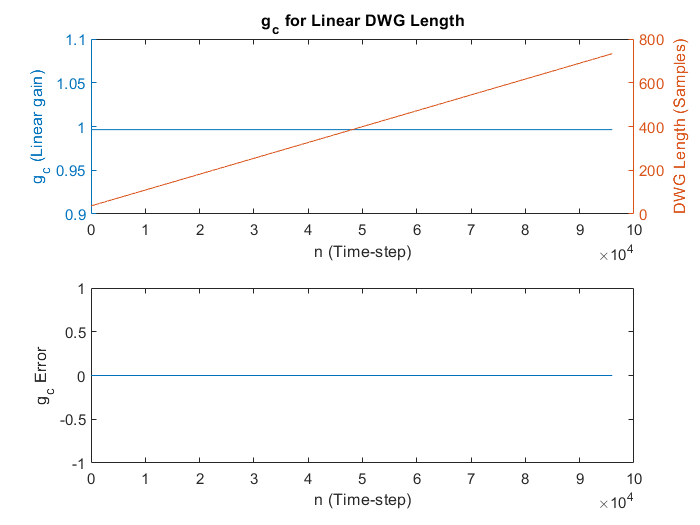
\includegraphics[scale=.45]{./images/plots/EnergyScalerLinearIncreasing.png}
    \caption{The Energy Scaler output in response to a linearly increasing input. The top plot illustrates the input/output signals as they evolve over time. The bottom figure illustrates correctness as the absolute error is 0.}
    \label{fig:EnergyScalerLinInc}
\end{figure}

\begin{figure}[h!]
    \centering
    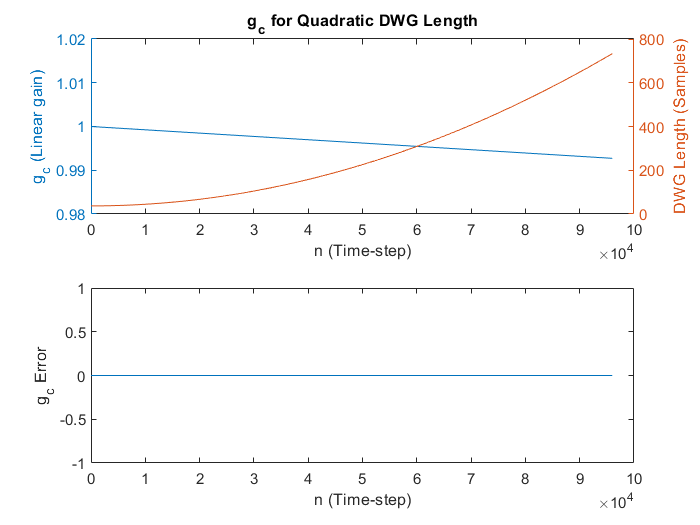
\includegraphics[scale=.45]{./images/plots/EnergyScalerQuadraticIncreasing.png}
    \caption{The Energy Scaler output in response to a quadratically increasing input. The top plot illustrates the input/output signals as they evolve over time. The bottom figure illustrates correctness as the absolute error is 0.}
    \label{fig:EnergyScalerQuadInc}
\end{figure}

\clearpage

\begin{figure}[h!]
    \centering
    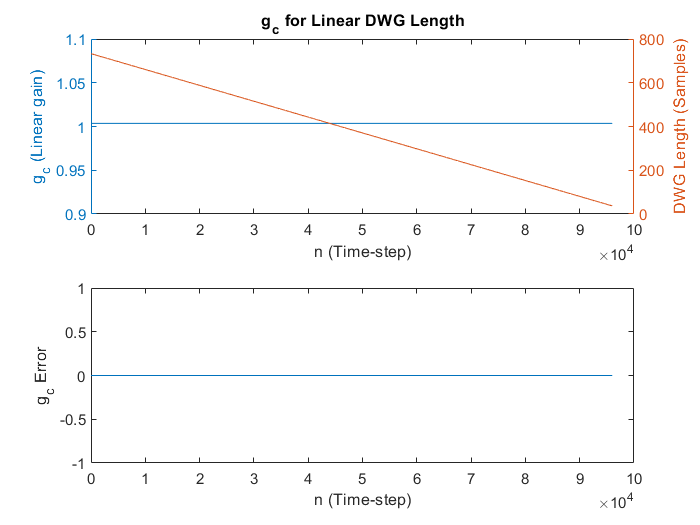
\includegraphics[scale=.57]{./images/plots/EnergyScalerLinearDecreasing.png}
    \caption{The Energy Scaler output in response to a linearly decreasing input. The top plot illustrates the input/output signals as they evolve over time. The bottom figure illustrates correctness as the calculated error is 0.}
    \label{fig:EnergyScalerLinDec}
\end{figure}

\begin{figure}[h!]
    \centering
    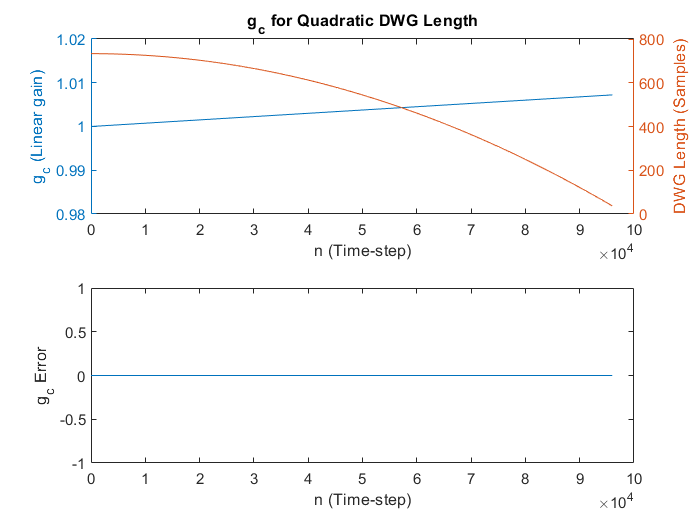
\includegraphics[scale=.57]{./images/plots/EnergyScalerQuadraticDecreasing.png}
    \caption{The Energy Scaler output in response to a quadraticly decreasing output. The top plot illustrates the input/output signals as they evolve over time. The bottom figure illustrates correctness as the calculated error is 0.}
    \label{fig:EnergyScalerQuadDec}
\end{figure}

\clearpage

\subsection{Loop Filter}
\label{subsec:Ch4LoopFilter}
As described in Sec.~\ref{sec:Ch2LoopFilter}, the loop filter was designed to approximate the various losses associated with vibrating string motion. It is a simple one-pole filter which uses a first-order polynomial approximation to generate $a$ and $g$ coefficients at various relative string length values (see Sec.~\ref{sec:Ch2LoopFilter}). Aspects of this approach have been examined in Sec.~\ref{sec:MinL} which illustrated that the filter itself is operational. The original paper provides the equations for the polynomial approximation as well as the polynomial coefficients. No frequency response plots are provided. In terms of the polynomial approximation, results are only provided for the first string. Accordingly the verification approach here involves recreating the original figures and relying on the fact the other coefficients have been copied correctly. Figures~\ref{fig:Fig18Orig} and~\ref{fig:Fig19Orig} show the original plots while Fig.~\ref{fig:Fig18Recon} and~\ref{fig:Fig19Recon} show the recreations respectively.

\begin{figure}[h!]
    \centering
    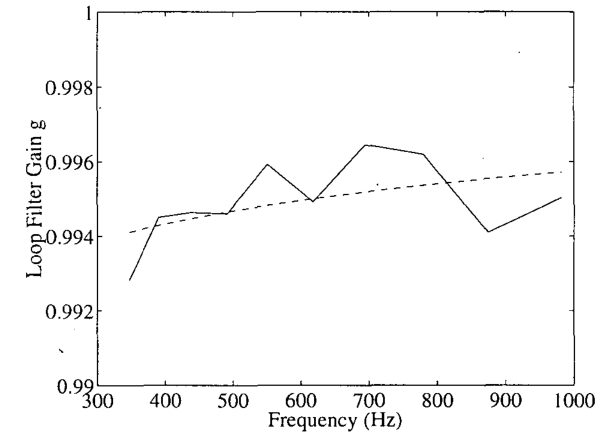
\includegraphics[scale=.50]{./images/plots/Figure18Orig.png}
    \caption{The loop gain \emph{g} for modeling string 1 (solid line) and first-order polynomial fit (dashed line) from \citetwo{valimaki_development_1998}.}
    \label{fig:Fig18Orig}
\end{figure}

\begin{figure}[h!]
    \centering
    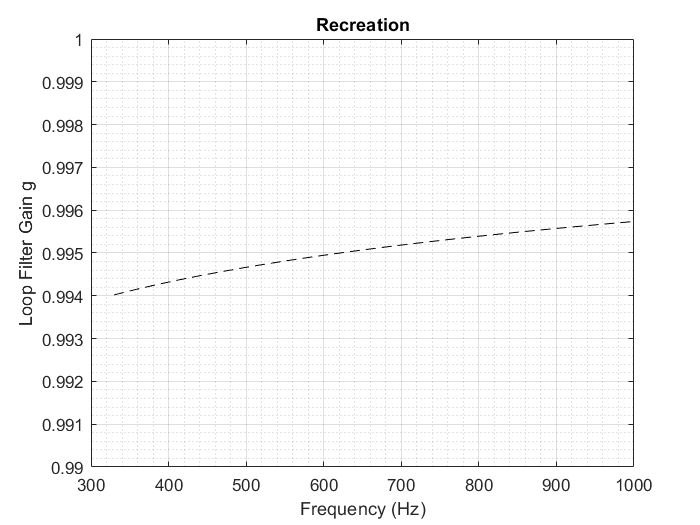
\includegraphics[scale=.50]{./images/plots/Figure18Recon.png}
    \caption{The loop gain \emph{g} polynomial for string 1 used in the slide synthesis model from this thesis.}
    \label{fig:Fig18Recon}
\end{figure}

\clearpage

\begin{figure}[h!]
    \centering
    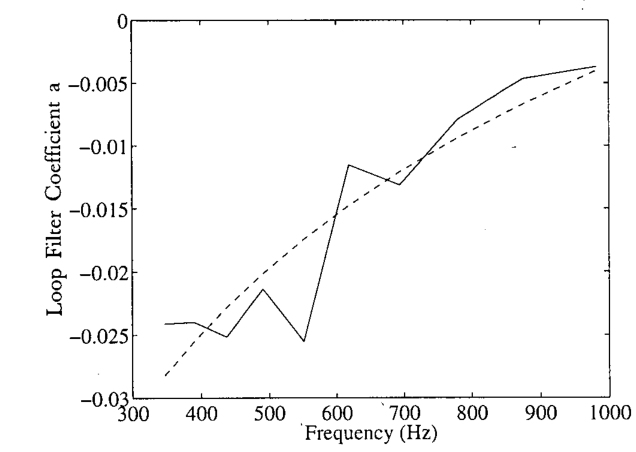
\includegraphics[scale=.75]{./images/plots/Figure19Orig.png}
    \caption{The loop-filter \emph{a} for string 1 (solid line) and first-order polynomial fit (dashed line) from \citetwo{valimaki_development_1998}.}
    \label{fig:Fig19Orig}
\end{figure}

\begin{figure}[h!]
    \centering
    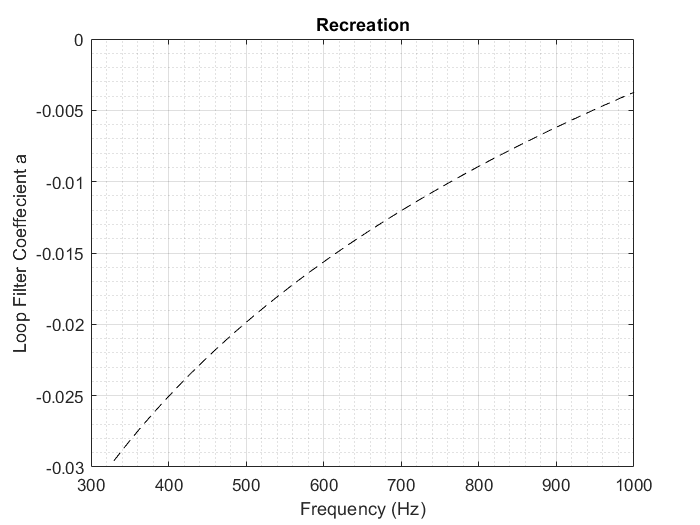
\includegraphics[scale=.65]{./images/plots/Figure19Recon.png}
    \caption{The loop-filter \emph{a} polynomial for string 1 used in the slide synthesis model from this thesis.}
    \label{fig:Fig19Recon}
\end{figure}

\clearpage

\subsection{String Digital Waveguide}
The string digital waveguide model was first verified to be free from transients and artifacts. This was achieved by running a series of sweeps on the relative length signal across its valid value range. After this was ensured, the tuning accuracy was verified via parabolic spectral interpolation as outlined in \citetwo{smith_spectral_nodate}. This method relies on computing the Discrete Fourier Transform (DFT) of the signal to sample its spectrum at N evenly spaced analysis frequencies. As a result, these analysis frequencies are harmonically related.

Ideally it would be best to have the harmonics generated by the string match the analysis frequencies. This would mitigate spectral leakage and reduce the need for interpolation in general. The fundamental frequency of the synthesized pitch was selected to align with a DFT bin but also be high enough so that several DFT bins exist in between the different harmonics. This is another method for mitigating spectral leakage. A lower fundamental frequency would produce a much more spectrally dense sound, which would be harder to get a clean estimate for.

The initial assumption in the algorithm development was that the strongest resonance present in the signal would be the fundamental frequency. In practice this was not the case, likely due to the initial waveform being initialized by noise as well as the non-idealities in the Loop Filter's magnitude response. The assumption had to be modified and a search range of the algorithm introduced. This search range is limited to $1.5*F_{0_{bin}}$, where $F_{0_{bin}}$ is the DFT bin associated with the synthesized sound. Other reasons for violations of the assumption could include the non-constant phase delay of both the loop as well as interpolation filter causing the frequencies to not all experience the same travel time and create a slight shift away from a perfectly harmonic signal.

To analyze the test signal, the following Short-Time Fourier Transform (STFT) analysis parameters were used:
\begin{itemize}
    \item Window Type = Hamming
    \item $Fs = 48,000$ Hz
    \item $N = 4096$
    \item Overlap = 75%
    \item Window length = 12 ms = 576 samples
\end{itemize}

The DWG was configured to generate a signal with a fundamental frequency corresponding with $F_{0_{bin}} = 100$, or 1,171.9 Hz. Following the method described in \citetwo{smith_spectral_nodate}, the calculated bin error was $8.3499 \times 10^{-5}$, which in Hertz is $9.7850 \times 10^{-4}$ Hz. As this is extremely small, the tuning was considered to be accurate and verified. Figures~\ref{fig:DWGInterpBins}-\ref{fig:DWGInterpSpec} illustrate this process.

\begin{figure}[h]
    \centering
    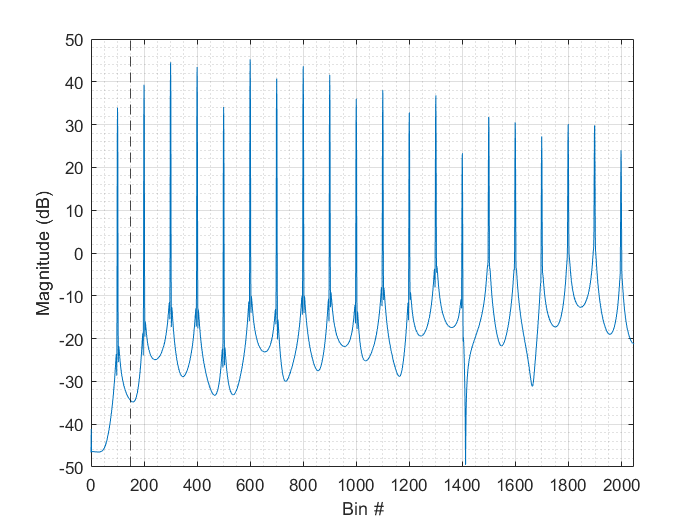
\includegraphics[scale=.65]{./images/plots/StringDWGInterpBins.png}
    \caption{The DFT of the tone produced for tuning verification. Note the upper harmonics which surpass the fundamental in strength. The dashed-black line indicates the upper search limit.}
    \label{fig:DWGInterpBins}
\end{figure}

\begin{figure}[h!]
    \centering
    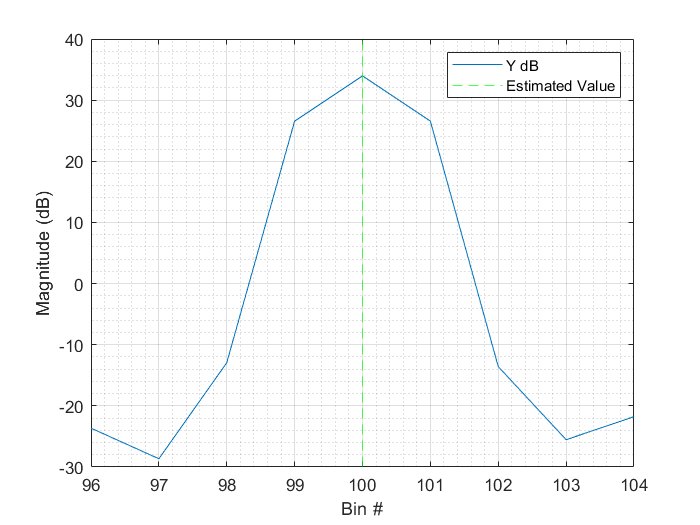
\includegraphics[scale=.58]{./images/plots/StringDWGInterpBinsZoom.png}
    \caption{A close-up of Fig.~\ref{fig:DWGInterpBins} near the estimated value.}
    \label{fig:DWGInterpBinsZoom}
\end{figure}

\begin{figure}[h!]
    \centering
    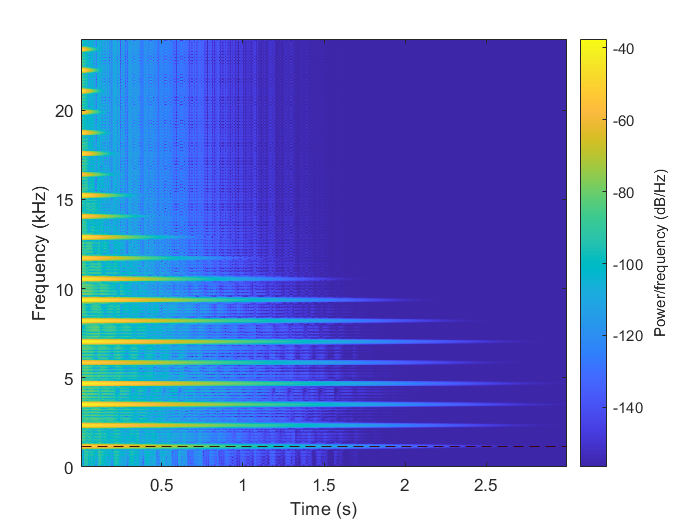
\includegraphics[scale=.58]{./images/plots/StringDWGInterpSpec.png}
    \caption{The spectrogram for the synthesized verification tone. The black dashed line is the estimation of fundamental. Note how the fundamental is not the strongest harmonic in the signal.}
    \label{fig:DWGInterpSpec}
\end{figure}

\section{Slide Synthesizer}
After all the individual components had been verified, a series of tests were run to check the overall functioning of the slide synthesizer. These tests were not meant to necessarily by physically accurate or musically useful, but purely as an approach to benchmark its basic behavior and determine the relationships between the CSG and DWG sound components. These were run with the different combinations of noise sources and harmonic accentuators as well as on the different string types. 

The testing scenarios are:
\begin{enumerate}
    \item Basic pluck with no slide motion
    \item Sliding up/down one fret over three seconds
    \item Sliding up/down three frets over one second
    \item Sliding up/down five frets over .5 seconds
    \item Sliding up/down extremes of relative string length
    \item Narrow/wide vibrato
\end{enumerate}
The output files and spectrograms were generated using the Noise Pulse Train and Harmonic Resonator Bank configuration using a mixture of the different strings. The filenames are \emph{SlideSynth-Test-\#-direction.wav}, where \emph{\#} is replaced with the corresponding test number and \emph{direction} is either up or down.

Figures~\ref{fig:VibratoWideSpec} and~\ref{fig:VibratoNarrowSpec} show the spectra from the different vibrato tests (case \#6). These are shown as they illustrate correctness of the more basic tests due to their comparative complexity. As can clearly be seen, the harmonics follow a sinusoidal trajectory corresponding to the parameters of the specified vibrato. The variations in the contact sound intensity can be seen as well. As is also shown, the contact sound dominates the spectrum as the string dies out, which is similar to what happens in the physical world.

\begin{figure}[h!]
    \centering
    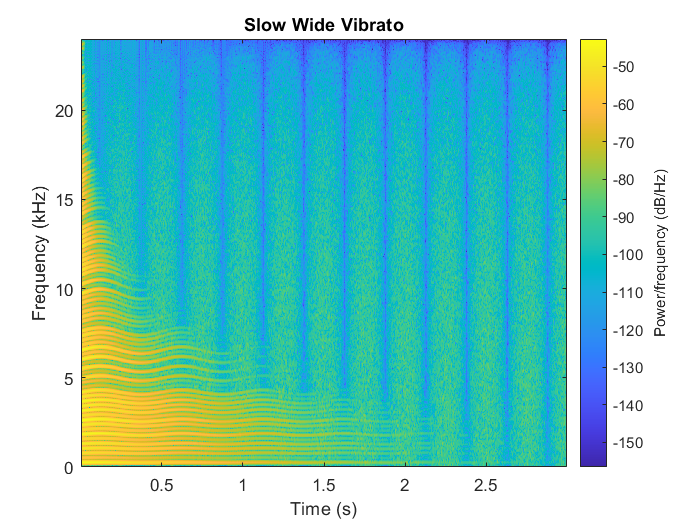
\includegraphics[scale=.55]{./images/plots/VibratoWideSpec.png}
    \caption{The spectrogram corresponding to the wide vibrato test. Note how both the harmonics and contact sounds respond corresponding to the sinusoidal relative string length.}
    \label{fig:VibratoWideSpec}
\end{figure}

\begin{figure}[h!]
    \centering
    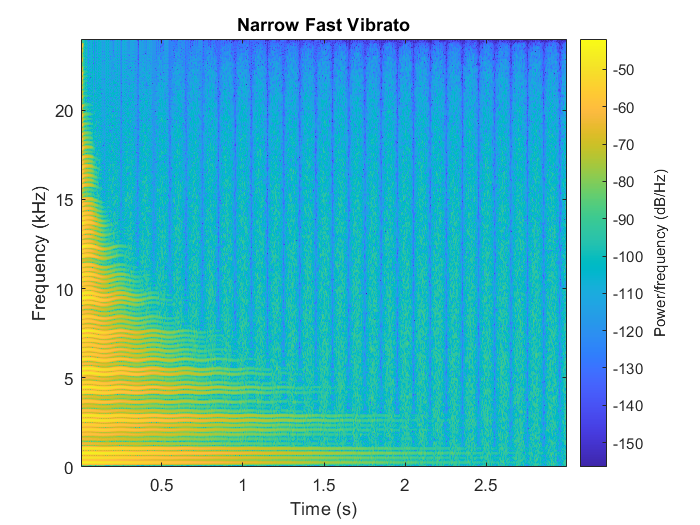
\includegraphics[scale=.55]{./images/plots/VibratoNarrowSpec.png}
    \caption{The spectrogram corresponding to the narrow vibrato test. Note how both the harmonics and contact sounds respond corresponding to the sinusoidal relative string length.}
    \label{fig:VibratoNarrowSpec}
\end{figure}

\section{Real-Time Feasibility}
The model used in this chapter is implemented in MATLAB due to its rich feature set related to digital signal processing which allows for easier verification of the implementation. The MATLAB implementation is not configured to run in real-time. However, it entirely seems feasible that the model could easily be implemented in real-time based on previous results. The model which serves as the basis for this thesis, described in \citetwo{pakarinen_virtual_2008} and \citetwo{puputti_real-time_2010}, is shown operating in real-time in the following video: \url{https://www.youtube.com/watch?v=aIJ-8kd8rFs}. The implementation is  in Pure Data and includes 6-strings simultaneously to recreate a full-guitar. Additionally, the computer is running image recognition software to facilitate gestural control as well as other software to simulate reverb and distortion. Given that this was achieved in 2010 using a 2.66 GHz Intel Pentium 4 CPU with 1 GB of RAM \citetwo{puputti_real-time_2010}, it entirely seems feasible that the model would be easily implemented using today's hardware, 13 years later, based on the rate at which computing power regularly increases.
\end{document}